\section{Training Data}
To equip Rex-Omni with both precise coordinate prediction capabilities and strong language understanding, we utilize two sources of training data: publicly available datasets and automatically annotated data generated by our custom-designed data engines.
\begin{table*}[t]
\centering
  \resizebox{1.0\linewidth}{!}{
    \begin{tabular}{c|c|c|c}
\hline
Task             & Output Format & Question Template Example                                                                                                                                                                                           & Datasets                                                                                                                                                                                               \\ \hline
Object Detection & Box           & Detect {[}PHRASE{]} in this image                                                                                                                                                                                   & \begin{tabular}[c]{@{}c@{}}APTv2~\cite{yang2023aptv2}, BDD100K~\cite{yu2020bdd100k}, DeepFashion~\cite{liu2016deepfashion}\\  DOTAv2~\cite{xia2018dota}, EgoObjects~\cite{zhu2023egoobjects}, FAIR-1M~\cite{sun2022fair1m}\\ HumanParts~\cite{li2018detector},  ImageNet-Part~\cite{he2022partimagenet} NuImages~\cite{caesar2020nuscenes}\\ PACO~\cite{ramanathan2023paco},  OpenImages~\cite{Datasets:OpenImages}, O365~\cite{shao2019objects365}\\ V3Det~\cite{wang2023v3det}, VisDrone~\cite{du2019visdrone}\end{tabular} \\ \hline
Object Referring & Box           & Detect {[}PHRASE{]} in this image                                                                                                                                                                                   & HumanRef, RefCOCOg                                                                                                                                                                                     \\ \hline
Visual Prompting & Box           & \begin{tabular}[c]{@{}c@{}}Given reference boxes {[}BOX{]} indicating one or more \\ objects,  find all objects with the same category\end{tabular}                                                                 & \begin{tabular}[c]{@{}c@{}}O365~\cite{shao2019objects365}, OpenImages~\cite{Datasets:OpenImages}, HierText~\cite{long2022towards} \\ CrowdHuman~\cite{shao2018crowdhuman}, SA-1B~\cite{TransF:SAM}, VisDrone~\cite{du2019visdrone} \\ FSCD147~\cite{nguyen2022few}\end{tabular}                                                                                         \\ \hline
OCR              & Box / Polygon & Detect all the text in box/polygon format and recognize them                                                                                                                                                        & \begin{tabular}[c]{@{}c@{}}Art~\cite{chng2019icdar2019}, HierText~\cite{long2022towards}, ICDAR2013~\cite{lucas2005icdar} \\ ICDAR2015~\cite{karatzas2015icdar},  LSVT~\cite{sun2019chinese}, RCTW~\cite{shi2017icdar2017}\\ ReCTS~\cite{zhang2019icdar}\\ SROIE~\cite{huang2019icdar}, TextOCR~\cite{singh2021textocr}\\ IDLOCR~\cite{biten2022ocr}, WildReceipt~\cite{sun2021spatial}\end{tabular}                                                      \\ \hline
Layout Groudning & Box           & Detect {[}PHRASE{]} in this image                                                                                                                                                                                   & \begin{tabular}[c]{@{}c@{}}DocLayNet~\cite{pfitzmann2022doclaynet}, PubLayNet~\cite{zhong2019publaynet}, TableBank~\cite{li2020tablebank} \\ M6Doc~\cite{cheng2023m6doc}, CDLA~\cite{li2021cdla}, TabRecSet~\cite{yang2023large}\end{tabular}                                                                                                     \\ \hline
GUI Grounding    & Box / Point   & Detect/Point to element {[}PHRASE{]}                                                                                                                                                                                & Os-Atlas~\cite{wu2024atlas}, UI-RefExp~\cite{bai2021uibert}, ShowUI~\cite{lin2024showui}                                                                                                                                                                            \\ \hline
Pointing         & Point         & Point to {[}PHRASE{]}                                                                                                                                                                                               & Pixmo-point~\cite{deitke2024molmo}                                                                                                                                                                                            \\ \hline
Affordance       & Point         & Point to {[}PHRASE{]}                                                                                                                                                                                               & AGD20K~\cite{luo2022learning}                                                                                                                                                                                                 \\ \hline
Spatial Referring       & Point         & Point to {[}PHRASE{]}                                                                                                                                                                                               & RefSpatial~\cite{zhou2025roborefer}                                                                                                                                                                                                 \\ \hline
KeyPointing      & Box \& Point  & \begin{tabular}[c]{@{}c@{}}Can you detect each {[}PHRASE{]} in the image \\ in box format, and then provide the coordinates of \\ its {[}KEYPOINT{]} as {[}x0, y0{]}? Output the \\ answer in JSON format.\end{tabular} & \begin{tabular}[c]{@{}c@{}}AP10K~\cite{yu2021ap}, APT36K~\cite{yang2022apt}, COCO-Keypoint~\cite{Datasets:MSCOCO} \\ MacaquePose~\cite{labuguen2021macaquepose}, HumanArt~\cite{ju2023human}, MPII~\cite{andriluka20142d}\\ OCHuman~\cite{zhang2019pose2seg}, CrowdPose~\cite{li2019crowdpose}\end{tabular}                                                                               \\ \hline
\end{tabular}}
  \caption{Publicly available training datasets used by Rex-Omni, covering tasks such as object detection, referring, prompting, OCR, grounding, pointing, affordance, and keypointing, with outputs including boxes, points, polygons, and JSON-formatted keypoints.}
  \label{tab:Public_dataset}
  \vspace{-2mm}
  \end{table*} 

\subsection{Public Datasets}
In Table \ref{tab:Public_dataset}, we enumerate the publicly available datasets leveraged for Rex-Omni's training across various subtasks, including Object Detection, Object Referring, Visual Prompting, OCR, Layout Grounding, GUI Grounding, Pointing, Affordance Grounding, Spatial Referring, and Keypointing. For each of these tasks, a set of question templates was defined to construct corresponding question-answer (QA) pairs. In total, approximately 8.9 million public data samples were utilized.


\subsection{Data Engines}

Effective training of Rex-Omni necessitates learning a fine-grained mapping between its 1,000 quantized coordinate tokens and the continuous pixel space of images. This capability demands a substantially larger volume of high-quality training data than what is conventionally available in existing public datasets. Moreover, while many public datasets offer category-level annotations, those providing richer, instance-level semantic grounding (e.g., referring expressions) remain scarce in both scale and diversity. To address these limitations, we developed a dedicated suite of data engines engineered to generate high-quality, large-scale training data specifically tailored for fine-grained spatial reasoning and complex language grounding tasks.

\begin{figure*}[t]
    \centering
    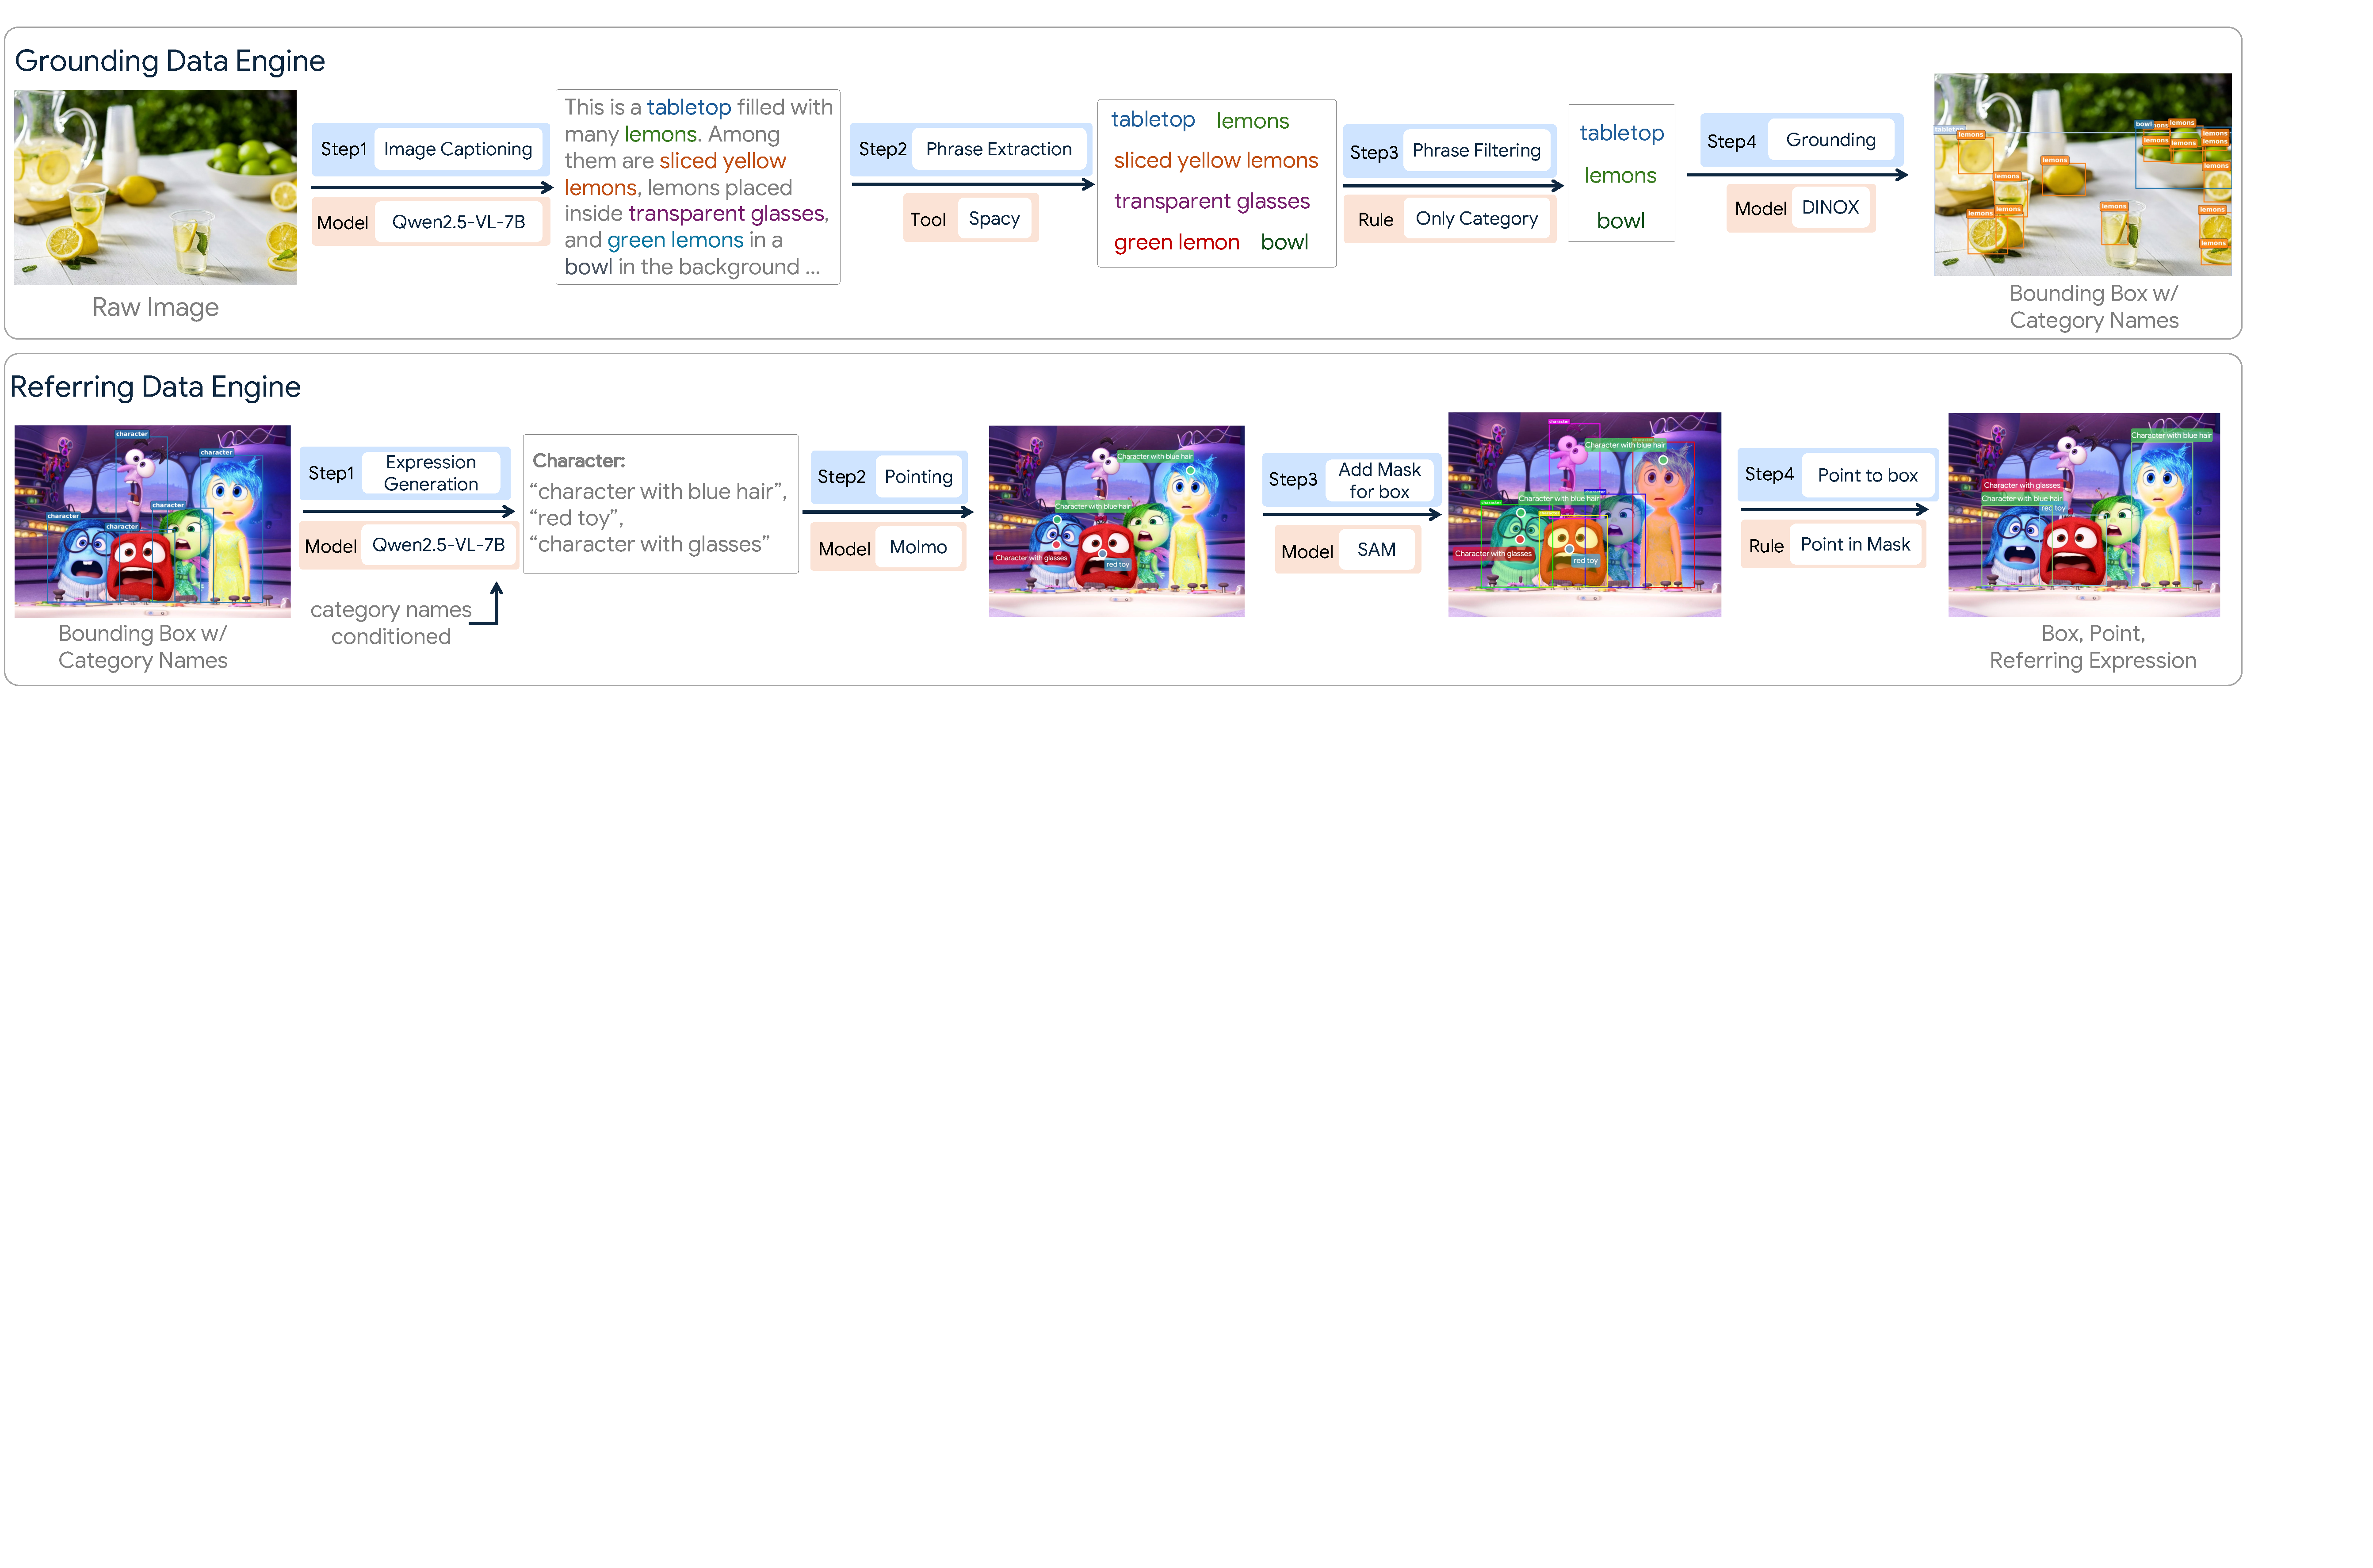
\includegraphics[width=\textwidth]{figures/data_engine.pdf}
    \caption{Pipelines of our two primary data engines. The figure illustrates the processes of the Grounding Data Engine (top) and the Referring Data Engine (bottom), which are custom-designed to produce extensive, high-quality grounding and referring data for Rex-Omni's training.
}
    \label{fig:data_engine}
\end{figure*}


\subsubsection{Grounding Data Engine}

A common strategy for constructing large-scale detection datasets is to develop a grounding data engine~\cite{jiang2024t, ren2024dino, ren2024grounding, cheng2024yolo, peng2023kosmos2}, which typically involves generating image captions, extracting candidate phrases, and using a grounding model (e.g., Grounding DINO) to assign bounding boxes to those phrases. In contrast to prior approaches, we introduce a phrase filtering stage into the pipeline to improve annotation quality. Specifically, our annotation process consists of the following four stages:

\begin{itemize}
    \item \textbf{Image Captioning:} We begin by generating descriptive captions for each image using Qwen2.5-VL-7B-Instruct. These captions provide natural language descriptions of the visual content, typically covering multiple objects within the scene.
    \item \textbf{Phrase Extraction:} We then apply the SpaCy\footnote{\url{https://spacy.io/}} NLP toolkit to extract noun phrases from the generated captions. These phrases may include basic class names (e.g., tabletop, lemon) as well as more specific descriptions (e.g., sliced yellow lemons, green lemons).
    \item \textbf{Phrase Filtering:} This step marks a key departure from prior approaches. To minimize data ambiguity, we remove noun phrases containing descriptive attributes such as adjectives (e.g., green lemon is discarded, while lemon is retained). The rationale is that current grounding models struggle to accurately interpret such descriptive expressions, often detecting all instances of a category regardless of the modifier. For instance, the phrase green lemon may incorrectly trigger detections of all lemons, thereby introducing significant labeling errors.
    \item \textbf{Phrase Grounding:} Finally, we use DINO-X \cite{ren2024dino}, an open-vocabulary object detector, to produce bounding boxes corresponding to the filtered phrases.
\end{itemize}

For this data engine, images are primarily sourced from the COYO~\cite{kakaobrain2022coyo-700m} and SA-1B~\cite{TransF:SAM} datasets. We apply rigorous preprocessing, including discarding low-resolution images and filtering content labeled as NSFW. This process yields a curated dataset of approximately 3 million images, each annotated with high-quality grounding labels.

\subsubsection{Referring Data Engine}

Unlike detection or grounding data, which primarily emphasize object category names, referring data necessitate semantically richer natural language descriptions, exemplified by phrases like “a man in a yellow shirt”. The RexSeek~\cite{jiang2025referringperson} study underscores that high-quality referring annotations should accommodate a single referring expression mapping to multiple instances, thereby fostering the model's ability to learn flexible and context-aware reference grounding. However, RexSeek's reliance on manual annotation renders it labor-intensive and inherently unscalable. To address this limitation, we design a fully automated referring data engine capable of generating large-scale referring data without human supervision.

\begin{itemize}
    \item \textbf{Expression Generation:} Given an image annotated with bounding boxes and corresponding category labels, we prompt Qwen2.5-VL-7B with the image and category information to generate a set of referring expressions. Each expression is designed to naturally describe an object category present in the image, mimicking human-like descriptions.
    \item \textbf{Pointing:} For each generated referring expression, we employ Molmo~\cite{deitke2024molmo}, a state-of-the-art referring model, to produce the corresponding spatial point. Although Molmo outputs only point-level predictions, it exhibits strong performance in understanding and grounding referring expressions.
    \item \textbf{Mask Generation:} We apply SAM~\cite{TransF:SAM} to generate a mask for each ground-truth bounding box in the image.
    \item \textbf{Point-to-Box Association:} Each point produced by Molmo is aligned with a SAM-generated mask. When a point lies within a mask, the corresponding bounding box is linked to the referring expression, thereby grounding the language in the object region.
\end{itemize}

For this data engine, we use images from O365~\cite{shao2019objects365}, OpenImages~\cite{Datasets:OpenImages}, and additional data generated by our Grounding Data Engine. Through this pipeline, we obtain approximately 3 million images with automatically generated referring annotations.

\subsubsection{Other Data Engines}
In addition to grounding and referring data, we develop two relatively lightweight data engines to generate datasets for pointing and OCR tasks.

\begin{itemize}
    \item \textbf{Pointing Data Engine:} Point-level supervision offers an efficient alternative to bounding boxes, particularly when object boundaries are ambiguous or difficult to delineate (e.g., edges, whitespace, or fine structures). To derive point annotations from box-level supervision, we adopt a geometry-aware strategy. Given a bounding box, SAM is first used to obtain the corresponding segmentation mask. We then compute the minimum-area enclosing rotated rectangle of the mask and take the intersection of its diagonals as the candidate point. If this point lies within the mask, it is designated as the point annotation for the box. Through this conversion, we obtain approximately 5 million point-level samples from existing detection datasets as well as from the outputs of our grounding and referring data engines.
    
    \item \textbf{OCR Data Engine:} PaddleOCR\footnote{\url{https://github.com/PaddlePaddle/PaddleOCR}} is utilized to annotate images containing textual content, extracting both polygonal boundaries of text regions and their corresponding transcriptions. For each extracted polygon, the minimum enclosing axis-aligned rectangle is subsequently computed to serve as its bounding box representation. Images are sourced from the COYO dataset, yielding approximately 2 million OCR-annotated samples.
\end{itemize}

In total, combining publicly available datasets and data generated by our annotation pipelines, we obtain 22 million high-quality annotated images for training.